\documentclass[a4paper,12pt]{article}
\usepackage{multicol}             % Escritura en columnas
\usepackage{amsmath}              % Matemáticas
\usepackage{musluatex}            % Musicología
\usepackage{booktabs}             % Tablas estéticas
\usepackage{float}                % para opción [H] en flotantes
\usepackage[hidelinks]{hyperref}  % Enlaces en referencias
\usepackage{tcolorbox}            % Cajas de color con título
\newtcolorbox{caja}[1]
{colback=black!5!white,colframe=gray!75!black,fonttitle=\bfseries,title={#1}}

\begin{document}
\title{Análisis de escalas}
\author{Pablo Herrera}
\date{\today}
\maketitle
\begin{abstract}
El presente artículo expone un método de análisis de escalas musicales a partir de los conceptos de \emph{distancia acústica} y \emph{distancia energética} entre los sonidos y la \emph{pertenencia} de los grados respecto a una tónica. Con él, en una escala dada se pueden develar las alianzas y las tensiones internas entre notas que perfilan características de las músicas surgidas de ella.
\end{abstract}
\tableofcontents
\begin{multicols}{2}
\section{Distancias}\label{sec:distancias}

  Cuando se habla de distancia entre dos sonidos muy habitualmente pensamos que un intervalo compuesto de más \emph{cents} o semitonos tiene más distancia entre sus componentes que otro intervalo con menos \emph{cents} o semitonos. Por ejemplo, decimos que en una quinta justa, de 702 \emph{cents} o 7 semitonos, hay más distancia entre los sonidos que la conforma que en una segunda mayor, de 204 \emph{cents} o 2 semitonos. O dicho de otro modo, mientras menos diferencia de frecuencia exista entre los sonidos del intervalo, más cercanía hay entre ellos. Sin embargo, cambiando hacia una óptica acústica, si observamos la relación entre \emph{do} y \emph{sol} respecto a los armónicos en común entre ambas notas, y hacemos lo propio entre \emph{do} y \emph{re}, notaremos que armónicos más cercanos a las fundamentales (tercer armónico de \emph{do} y segundo de \emph{sol}) son el invisible hilo que une a esas notas, mientras que entre \emph{do} y \emph{re} (noveno armónico de la nota grave y octavo de la nota aguda) ese hilo, construido con armónicos menos audibles y con menor intensidad, hace que la relación de segunda mayor sea \emph{más lejana} que la relación de quinta justa.

  Es más común pensar las distancias entre sonidos del primer modo porque se hace cotidiano, tanto al cantar como al tocar la mayoría de instrumentos musicales, que moverse de \emph{do} a \emph{re} requiere, por lo general, menos energía que la necesaria para moverse de \emph{do} a \emph{sol}. Distancia energética y distancia acústica son dos cosas diferentes: mientras energéticamente \emph{re} está más cerca de \emph{do}, acústicamente \emph{sol} es, de hecho ---luego del unísono y la octava---, la nota más cercana a \emph{do}. \emph{Distancia energética} y \emph{distancia acústica} son los dos conceptos que están en la base del análisis de escalas. Mientras la cercanía energética es la que define uno de los dos arquetipos musicales más importantes, la escala, la cercanía acústica da lugar al otro arquetipo musical sobresaliente, el arpegio. En un arpegio mayor, fundamental, quinta y tercera conforman la tríada de notas más cercanas entre sí\footnote{Aunque entre la tercera y la quinta no existe una armonía donde una sea la fundamental de la otra, sino que ambas tienen en la fundamental de la tríada mayor su posibilidad de estabilidad. Una tercera menor no se estabiliza sino con la presencia de su fundamental.}, y en la escala se manifiesta el movimiento melódico en el que se gradúan los cambios energéticos necesarios para llevar a plano sensible sonidos sucesivos. O dicho de otro modo, la escala representa el movimiento melódico donde se expresa en su orden la mayor cercanía energética entre los sonidos que la componen, y el arpegio es el conjunto de notas acústicamente más cercanas entre sí.

\section{Movimientos}\label{sec:movimientos}

  Existen tres formas posibles de relación entre dos notas:
  \begin{enumerate}
    \item Fundamental con un representante de un armónico de dicha fundamental.
    \item Un representante de un armónico con su fundamental.
    \item Dos notas que ninguna es representante de un armónico de la otra.
  \end{enumerate}

  Cuando una fundamental se dirige a una nota representante de un armónico suyo, el efecto sonoro es el contrario al de un movimiento cadencial. Es un movimiento melódico que invita a la continuación, una no-cadencia, una representación de lo abierto.

  Por ejemplo, \\ \musncp{c'1 g' \bar "||" c' e' \bar"||" c'' g' \bar "||" c'' e' \bar "||"}  son movimientos melódicos abiertos, no-cadenciales.

  Cuando una nota representante de un armónico de una fundamental se dirige a ella, se genera la sensación opuesta a la del caso anterior, es decir es un movimiento melódico cadencial, una representación de lo cerrado.

  Por ejemplo, \\ \musncp{g'1 c' \bar "||" e' c' \bar "||" g' c'' \bar "||" \mark "*)"e' c'' \bar "||"} son movimientos melódicos cerrados, cadenciales.\footnote{La sexta menor, marcada con *) en el ejemplo, es acústicamente cercana mas no energéticamente, por lo que su poder cadencial queda comprometido.}

  Cuando las notas intervinientes en el movimiento melódico no son una fundamental de la otra, ocurre la mayor de las libertades melódicas, ya que no hay ninguna dependencia entre las notas intervinientes.

  Por ejemplo, \\ \musncp{e'1 g' \bar "||" g' e' \bar "||" e'' g' \bar "||" g' e'' \bar "||" }  son movimientos melódicos libres, semiabiertos o semicerrados, según el contexto. Esto es así porque \emph{mi} no es armónico audible de \emph{sol} y viceversa.

  Una aclaración final antes de pasar al análisis de escalas propiamente dicho: cuando una nota es representante de un armónico de otra con la que está conformando intervalo, decimos que ella tiene \emph{pertenencia} a esa otra nota.

\section{Pertenencia}\label{sec:pertenencia}
  Una escala con centro tonal es un conjunto de notas comprendidas en una octava que se relacionan con la tónica según su pertenencia o no a la serie de armónicos de dicha tónica. Expresado de otro modo, la tónica es, en cierta forma, la fundamental de la escala.

    \subsection{Una escala sin tensiones internas}\label{subsec:escala-sin-tensiones}
    La escala \hbox{\musncp{\relative{c'2 d4 e g a c2}},} por ejemplo, tiene en \musncp{d'} al armónico 9 de \hbox{\musncp{c'};} en \hbox{\musncp{e'},} al armónico 5 de la tónica; en \hbox{\musncp{g'},} al armónico 3; y en \hbox{\musncp{a'},} al décimo tercer armónico. Esto es importante porque cuando una nota es la representante de un armónico audible de la tónica, tiene, salvo en un caso ---el armónico 11---, la facultad de generar un movimiento cadencial hacia el centro tonal establecido. En este ejemplo, las notas \emph{re, mi, sol, la} son todas capaces de producir un movimiento melódico que produce en la percepción humana la sensación de cierre, de conclusión.
\end{multicols}

\begin{figure}[ht]
\centering
\begin{lilypond}[notime]
\relative {
  \mark \markup{\italic a)}
  d'1 c \mark \markup{\italic b)} \bar "||"
  e c \mark \markup{\italic c)} \bar "||"
  g' c \mark \markup{\italic d)} \bar "||"
  a c \bar "||"
}
\end{lilypond}
\caption{Movimientos melódicos cadenciales de notas con pertenencia a la tónica.}\label{fig:mov-cad}
\end{figure}

\begin{multicols}{2}
  El ejemplo \emph{a)} de la Figura~\ref{fig:mov-cad} muestra un movimiento cadencial muy fuerte, ya que la cercanía energética de \emph{re} a \emph{do} sumado a la relativa cercanía acústica (9:8) confluyen para producir tal fuerza.

  Los ejemplos \emph{b)} y \emph{c)} muestran los movimientos melódicos cadenciales propios de notas representantes de armónicos audibles cercanos dirigiéndose hacia la nota representante de su fundamental.

  Se podrá objetar que en \emph{d)} de la Figura~\ref{fig:mov-cad}, al ser \emph{la} un representante del armónico 13 de la tónica y al ser éste poco audible no hay razón para considerar al movimiento \musncp{a' c''} como cadencial. Sin embargo, tanto la tercera menor ascendente como la descendente son posibles movimientos cadenciales por cercanía energética. Se podría decir que ni \emph{la} es armónico de \emph{do} ni \emph{do} de \emph{la} y por lo tanto es un movimiento melódico libre, y lo es, pero el contexto de haber definido a \emph{do} como tónica convierte a éste en un movimiento cadencial.

    \subsection{Tensión interna en una escala}\label{subsec:tension}

    Tomemos ahora como modelo escalístico a analizar a la escala \hbox{ \musncp{\relative{c'2 d4 e f g a b c2}}.} En esta escala, tras comprobar la pertenencia de los grados a la tónica \emph{do}, notamos que uno de ellos carece tanto de cercanía acústica como de cercanía energética respecto a la tónica: el \grado{4} grado.
\end{multicols}

\begin{figure}[ht]
\centering
\begin{lilypond}[notime]
\score {
  <<
    \new Staff {
      \relative {
        \hide Stem
        c'2 d4 e f g a b c2
      }
    }
    \new Lyrics \lyricmode { "1"2 "9"4 "5" - "3" "13" "15" "2" }
  >>
}
\end{lilypond}
\caption{Pertenencia a la tónica de los grados de la escala de Do mayor. }\label{fig:pertenencia-do}
\end{figure}

\begin{multicols}{2}
    En rigor de verdad, el \grado{4} grado no es lejano acústicamente de la tónica, pero \emph{do} no es la tónica de \emph{fa}, sino al revés: la tónica de la tonalidad es el tercer armónico del \grado{4} grado, algo así como que \emph{fa} es la tónica de \emph{do}. Por esto hay conflicto entre el centro tonal establecido y su \grado{4} grado, porque éste tiende a convertirse en una nueva tónica, compitiendo directamente por el poder dentro de la escala con el \grado{1} grado.

    \subsection{Una escala con más tensiones internas}\label{subsec:esc-mas-tensiones}
    Habiendo visto brevemente las escalas pentatónica y mayor, veamos ahora, también brevemente, al modo menor. La escala \musncp{\relative{\key c \minor c'2 d4 es f g aes bes c2}} con su \grado{7} grado mutable con fines cadenciales y su \grado{6} mutable también, principalmente con fines de conectividad melódica entre el \grado{5} y \grado{7}, posee más que los dos semitonos que tiene la escala mayor, \emph{y donde hay semitonos pueden pasar cosas importantes}. A los semitonos existentes entre \grado{2} y \grado{3} y entre \grado{6} y \grado{5} se suma, vía alteración ascendente, el semitono entre \grado{7} y \grado{8} (o \grado{1}) \hbox{\musncp{\key c \minor b' ( c'' )}.} Al ser el \grado{3} una nota que no representa a un armónico audible de \emph{do}, él no tiene pertenencia a la tónica, no es, por así decirlo, pariente de la tónica; sin embargo el \grado{1} arma alianza con el \grado{3}, junto al \grado{5} ---y con él indirectamente también con el \grado{7} ascendido, aliado natural del \grado{5} por ser representante de su armónico 5--- para conformar el grupo de notas que adhieren al \grado{1} como tónica de la escala. Pero antes de seguir hablando del \grado{3} grado, realicemos el análisis de pertenencia de los grados de la escala menor respecto a su tónica:
\end{multicols}

\begin{figure}[ht]
\centering
\begin{lilypond}[notime]
\score {
  <<
    \new Staff \relative c' {
        \key c \minor
        \hide Stem
        c2 d4 ( es ) f g ( aes ) bes \bar"!" a4 b ( c2 ) \bar "||"
    }
    \new Lyrics \lyricmode {
      "1"2 "9"4 "-" "-" "3" "-" "7" "13" "15" "2"2
    }
  >>
}
\end{lilypond}
\caption{Pertenencia de los grados del modo menor a la tónica.}\label{fig:pertenencia-menor}
\end{figure}

\begin{multicols}{2}
    Como se puede observar en la Figura~\ref{fig:pertenencia-menor}, los grados \grado{3}, \grado{4} y \grado{6} carecen de pertenencia a la tónica, por lo que son potenciales rivales de ella en la lucha por ocupar el centro del sistema. Ahora sí, dicho esto, podemos seguir hablando del \grado{3} grado.

    El semitono \musncp{\key c \minor d' ( es' )} hace del \emph{mi\bemoltxt}, sumado a la no pertenencia de esa nota a la tónica, un potencial centro tonal al cual se llega sin esfuerzo alguno. Todas las condiciones están dadas para que el \grado{3} grado se convierta en el nuevo rey: la tónica no tiene sino inventada por alteración ficta una sensible, una nota energéticamente cercana que se dirija a ella, y el \grado{3} grado sí. Además, el \grado{7} y el \grado{5}, naturales aliados suyos, están también presentes en la escala para conformar el grupo de notas \musncp{es'2 g' bes'} que juntas empoderan a \emph{mi\bemoltxt}.

    Pero el \grado{3} grado no las tiene todas consigo para llegar al poder tonal: el \grado{6} grado, el cual también tiene en sus alrededores un semitono que lo favorece, \hbox{ \musncp{g' ( aes' )},} y para colmo de bienes para él, es el representante de la fundamental de \emph{mi\bemoltxt}. Lo acá descripto no es otra cosa que lo que sucede entre la tónica y el \grado{4} grado en el modo mayor, sólo que en el modo menor, lógicamente por ser tonalidad relativa, ocurre entre \grado{3} y \grado{6}.

    Por último, y no por eso menos significativo en el esquema de poder del modo menor, se encuentra, con todas sus ansias de poder, el \grado{4} grado. Esta vez la anatomía interválica de la escala no lo favorece, como sí sucede en el modo mayor, con un semitono que le conceda mayor peso, pero sigue teniendo, al igual que en el modo mayor, toda la ascendencia sobre el \grado{1} grado.

  \section{Intervalos y afinación}\label{sec:intervalos-afinacion}
  Son intervalos muy diferentes los que se usan estando en una afinación concordante con los armónicos de los sonidos como lo es la \emph{entonación justa} de los que se utilizan estando en una afinación como la del \emph{igual temperamento}. El hecho de llamar \emph{tercera mayor} tanto a un intervalo de proporción $5:4$ como a otro surgido de $2^{\frac{4}{12}}$ es muy significativo y sin dudas la raíz de tratar a esos dos intervalos tan diferentes como si fuesen el mismo intervalo.\footnote{Mientras $5:4=1.2500$, $2^{\frac{4}{12}}=1.2599$, lo que, expresado en \emph{cents}, es $386.31$ para el intervalo $5:4$ y $400.00$ para el intervalo $2^{\frac{4}{12}}$. La tercera mayor igual temperada es casi 14 \emph{cents} más grande que la tercera mayor de la afinación justa.} En un intervalo $5:4$ hay una dependencia del sonido agudo respecto al grave por ser éste representante de la fundamental de aquél, mientras que en un intervalo $2^{\frac{4}{12}}$ los sonidos que lo conforman carecen de la cercanía acústica que haga de uno de ellos un sonido dependiente del otro; son dos sonidos que se relacionan «en igualdad de condiciones», ninguno de ellos es un representante de un armónico del otro. La libertad de movimiento que tiene todo intervalo dentro del \emph{igual temperamento} es total, ya que no hay movimientos melódicos cadenciales y no-cadenciales ---todos pueden ser cadenciales y todos pueden ser no-cadenciales--- sino solamente movimientos melódicos libres, como los que ocurren entre armónicos de una fundamental ausente. En los \emph{temperamentos irregulares} como los barrocos (\textsc{Vallotti}, \textsc{Wercmeister}, etc.) estamos ante un escenario híbrido: en parte algunos intervalos permanecen puros mientras otros, de misma denominación, son acústicamente lejanos. En \textsc{Kirnberger III} ---uno de los más importantes y usados temperamentos del siglo XVIII--- se dan cuatro tipos de terceras mayores, de los cuales tres de ellas son proporciones que devienen en intervalos conformados por notas independientes, quedando únicamente una de las doce terceras mayores posibles como proporción $5:4$: la tercera mayor de la tríada de Do mayor. Escenario híbrido, pero ya bastante cerca de lo que plantea el \emph{igual temperamento}: la muerte de las relaciones interválicas conformadas por sonidos acústicamente cercanos.
\end{multicols}

  \begin{caja}{Notación de escalas e intervalos}
  { \label{caja:notacion-escalas} \footnotesize
    \texttt{Visto que el \emph{cent} es una unidad de medida cuyos números más sencillos coinciden con el igual temperamento ---los números redondos como 300, 500 o 1100 representan intervalos igual temperados--- y considerando que la escala \musncp{\relative {c'2 d e f g a b c}} no es la misma en afinación justa que en otro temperamento, se propone anotar las escalas no solamente con sus notas en el pentagrama, sino con la desviación en \emph{cents} respecto al igual temperamento que cada una de ellas tiene. El siguiente ejemplo muestra dos escalas completamente diferentes:}

    \begin{center}
      \textsc{Escala de Do mayor en afinación justa:}

      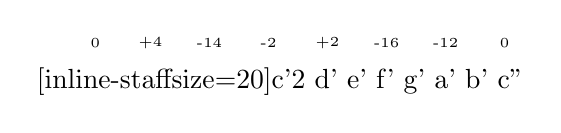
\begin{tikzpicture}[scale=1, transform shape]
        \node at (0,0){\musncp[inline-staffsize=20]{c'2 d' e' f' g' a' b' c''}};
        \node at (-2.35,0.5){\tiny 0};%do
        \node at (-1.65,0.5){\tiny +4};%re
        \node at (-0.9,0.5){\tiny -14};%mi
        \node at (-0.15,0.5){\tiny -2};%fa
        \node at (0.6,0.5){\tiny +2};%sol
        \node at (1.35,0.5){\tiny -16};%la
        \node at (2.1,0.5){\tiny -12};%si
        \node at (2.85,0.5){\tiny 0};%do
      \end{tikzpicture}

      \bigskip

      \textsc{Escala de Do mayor en temperamento igual:}

      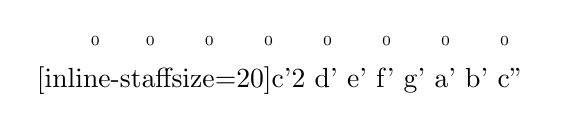
\begin{tikzpicture}[scale=1, transform shape]
        \node at (0,0){\musncp[inline-staffsize=20]{c'2 d' e' f' g' a' b' c''}};
        \node at (-2.35,0.5){\tiny 0};%do
        \node at (-1.65,0.5){\tiny 0};%re
        \node at (-0.9,0.5){\tiny 0};%mi
        \node at (-0.15,0.5){\tiny 0};%fa
        \node at (0.6,0.5){\tiny 0};%sol
        \node at (1.35,0.5){\tiny 0};%la
        \node at (2.1,0.5){\tiny 0};%si
        \node at (2.85,0.5){\tiny 0};%do
      \end{tikzpicture}
    \end{center}

    \texttt{Los intervalos pueden anotarse, en forma similar a las escalas, en pentagrama indicando también la desviación en \emph{cents} respecto al temperamento igual, o bien adoptar nombres más completos como 3M-IT para una tercera mayor igual temperada. También es posible decir \emph{Tercera mayor} solamente para el intervalo de proporción $5:4$ y para la relación interválica $2^{\frac{4}{12}}$ utilizar simplemente la forma popularizada por la teoría \emph{Pitch Class}, en la que +4, -4 o 4 son terceras mayores igual temperadas ascendente, descendente o armónica respectivamente. Lo que sin dudas es necesario es aclarar la precisión de la afinación de los sonidos conformantes del intervalo, porque en ello están las características, las propiedades de dicho intervalo.}
  }
  \end{caja}

\begin{multicols}{2}
  Ahora estudiaremos brevemente cómo el modo mayor (Jónico) pasa de ser estable en la antigüedad a inestable en la modernidad, y de cómo el modo menor (eólico) transitó un camino inverso, es decir de inicial inestabilidad hacia una posterior estabilidad, todo esto por causa del cambio de afinación desde la afinación justa y el temperamento mesotónico hacia los temperamentos irregulares y el temperamento igual.

  Tanto en una afinación justa (\textsc{Aristóxeno}) como en una afinación natural (espectral) la tercera mayor, por tener a la representante de la fundamental en el grave, es un intervalo muy estable, que tiende a la quietud. En el temperamento igual ese intervalo pierde esa propiedad, haciéndose un intervalo cuyo significado sonoro es de una movilidad intermedia.

  En un acorde triada mayor el aporte de la quinta a la sonoridad en su conjunto es mucho menor que el que hace la tercera. Si la quinta está perfectamente afinada y la tercera no, el acorde se desestabiliza; si, en cambio, la tercera gana en estabilidad, el acorde, aunque posea una quinta con cierta inestabilidad, también gana en estabilidad y quietud. Así, pues, tanto con la afinación justa como con la afinación espectral, en una tonalidad mayor la tercera mayor de un acorde de tónica otorga al complejo sonoro un alto grado de estabilidad. Al cambiar este intervalo en los temperamentos irregulares del siglo XVIII y en el igual temperamento, el mismo acorde pierde su antigua estabilidad. La consecuencia directa: el modo mayor ya no es estable como lo era por causa de la complejización del intervalo de tercera mayor y, consecuentemente, del acorde de tónica de la tonalidad mayor.
\end{multicols}

\begin{table}[ht]
  \centering
  \caption{Comparación de la 3M en las tres afinaciones.}\label{tab:3M}
  \begin{tabular}{@{}llll@{}}
  \toprule
  Intervalo               & Proporción  & Cociente  & Cents   \\ \midrule
  Tercera mayor A.J.      & $5:4$       & $1.2500$  & $386.3$ \\
  Tercera mayor espectral & $5:4$       & $1.2500$  & $386.3$ \\
  Tercera mayor T.I.      & $2^{4/12}$  & $1.2599$  & $400.0$ \\ \bottomrule
  \end{tabular}
\end{table}

\begin{multicols}{2}
  En la afinación justa, la tercera menor es compleja a pesar de que sus números parecen simples ($6:5$) debido a la ausencia de la fundamental (ausencia de un denominador 1, 2 o potencia de 2), o, dicho de otro modo, es un intervalo que «busca a su fundamental» ---ubicada a una tercera mayor por debajo de la nota grave como, por ejemplo, \musncp{f'2} en \hbox{\musncp{<a' c''>4}.} Esta característica de la tercera menor es heredada por el modo menor a causa de la fuerte influencia del intervalo en la conformación de la sonoridad del acorde de tónica, el cual se estabiliza con la presencia del \grado{6} grado de la tonalidad ---el acorde \musncp{<a' c'' e''>}, I de La menor, se estabiliza en \hbox{\musncp{<f' a' c'' e''>}.} En la afinación natural (espectral), la tercera menor respecto a la tónica aparece entre los armónicos 19 y 16 (proporción $19:16$). Es una relación interválica entre armónicos menos audibles, pero con la enorme ventaja de la estabilidad que le confiere la presencia de la fundamental. Su medida en \emph{cents} es $297.5$, y la tercera menor igual temperada, es de $300$ \emph{cents}.\footnote{Una diferencia de $\pm3$ \emph{cents} es auditivamente irrelevante ---aunque, hay que decirlo, un ser humano no oye únicamente con sus oídos.} Por este motivo, toda la inestabilidad que se percibe en el modo eólico con una afinación justa desaparece cuando se utiliza el igual temperamento o la afinación espectral, dándole al modo menor mucha más estabilidad en su acorde de tónica y, por lo tanto, a toda la tonalidad.
\end{multicols}

\begin{table}[ht]
  \centering
  \caption{Comparación de la 3m en las tres afinaciones.}\label{tab:3m}
  \begin{tabular}{@{}llll@{}}
  \toprule
  Intervalo               & Proporción  & Cociente & Cents   \\ \midrule
  Tercera menor A.J.      & $6:5$       & $1.2000$ & $315.6$ \\
  Tercera menor espectral & $19:16$     & $1.1875$ & $297.5$ \\
  Tercera menor T.I.      & $2^{3/12}$  & $1.1892$ & $300.0$ \\ \bottomrule
  \end{tabular}
\end{table}

\begin{multicols}{2}
  La pérdida de estabilidad del modo mayor y la ganancia de ella en el modo menor cuando el temperamento igual es el usado son características que fueron redirigiendo históricamente los rumbos de la composición musical.

  En el siglo XX se vuelve a poner sobre la mesa el tema del uso de los intervalos compuestos por notas acústicamente cercanas. \textsc{Julián Carrillo} ---compositor romántico y microtonal--- y la \emph{música espectral} dan testimonio de ello.

  En definitiva, las posturas de \textsc{Aristóxeno} ---mentor de la \emph{afinación justa}--- y \textsc{Pitágoras} ---precursor de los temperamentos regulares como el \emph{igual temperamento}--- en relación a la temática de la afinación en música no ha perdido vigencia a través de los tiempos hasta nuestros días, días en los que seguimos debatiéndonos entre las posibilidades combinatorias, las purezas interválicas y la búsqueda de la imposible perfección en un mundo en el que la quietud es utopía.
\end{multicols}

\begin{figure}[ht]
\centering
\begin{lilypond}[notime]
  \layout {
    \context {
      \Voice
      \consists Horizontal_bracket_engraver
    }
  }
  {
    \mark \markup{\italic "a)"}
    \hide Stem
    <c' e' g'>2 \bar "!"
    c'2 e' g' c'' \bar "||"
    \mark \markup{\italic "b)"}
    <<{ \stemDown \hide Stem c''2} \\ {\hide Stem <g'' f'>4}>> \bar "!"
    c''2\startGroup g'4\stopGroup f'\startGroup s c'2\stopGroup \bar "||"
  }
\end{lilypond}
\caption{Dos estructuras basadas en cercanía acústica.}\label{fig:dos-estructuras}
\end{figure}

\begin{multicols}{2}
\section{Estructuras}\label{sec:estructuras}
  \subsection{Arpegio}\label{subsec:arpegio}
  La cercanía acústica de los grados \grado{5} y \grado{3} respecto al \grado{1} propone, en una música que tenga como notas estructurales a estos tres grados, un juego bidireccional de los movimientos melódicos: abiertos cuando la línea melódica se dirige desde \grado{1} hacia \grado{3} o \grado{5}, y cerrados cuando la línea melódica direcciona sus movimientos desde los grados \grado{5} y \grado{3} hacia el \grado{1} grado. Mientras los movimientos melódicos se produzcan entre \grado{3} y \grado{5} el transcurrir melódico nos deposita en una zona de no-definición, de prolongación de lo abierto e irresuelto. Una baguala\footnote{Una baguala es una pieza musical característica de la zona de montaña del norte argentino (provincias de Salta y Jujuy) de carácter improvisatorio basada en una escala tritónica donde fundamental, quinta y tercera juegan acompañadas de una caja, instrumento de percusión también típico de esta región.}, que además de usar las notas de la estructura arpegio excluye a otras notas, desnuda y revela con más facilidad lo anteriormente dicho: \mus{\time 3/4 \relative c' {c4. 8 e4 g4. e8 g4 g4 e2}} es una frase que, estructuralmente se hace \musncp{\hide Stem c'2 e' g' e'} es decir un movimiento no-cadencial \musncp{c'2 e'} seguido de una prolongación de lo abierto en \musncp{e'2 g' e'} haciendo de toda la frase musical un fragmento de carácter abierto, irresuelto; el consecuente habitual de esta frase suele ser, típicamente, \mus{\time 3/4 \relative g'{g4. e8 g4 4. e8 c4 4 2 \bar "|."}} que cierra con el movimiento melódico cadencial \musncp{e'2 c'} el cual es antecedido por la prolongación de lo abierto con las notas\hbox{\musncp{g'2 e' g' e'}.}

  El fragmento \musncp{c'2 f'4 d' e'2 a'4 g'2}, desarrollo melódico ya dentro de un ámbito heptatónico, no es disímil en términos estructurales al antecedente del ejemplo de baguala precedente: \musncp{c'2 e' g'} siguen siendo las notas que sostienen ese tejido melódico y, por ser movimientos melódicos no-cadenciales, este fragmento también posee carácter abierto, no resolutivo. Si completamos la frase anterior con un posible fragmento como \musncp{g'2 f'4 e'2 d'4 b c'2} estamos, una vez más, ante una situación análoga al consecuente de la baguala: una estructura melódica \musncp{g'2 e' c'} que completa y cierra, por su carácter cadencial, la frase musical.

  Lo tritónico subyace en lo pentatónico, y lo pentatónico subyace en lo heptatónico. Las escalas analizadas brevemente en la sección~\ref{sec:pertenencia} son las que son justamente por la importancia estructural e histórica que ellas tienen en la música.

  \subsection{Tetracordios}\label{subsec:tetracordios}

  La cercanía acústica de los grados \grado{4} y \grado{5} respecto a la tónica \grado{1} es algo que se ve reflejado en innumerables manifestaciones culturales distantes entre sí tanto en tiempo como en espacio. Una de esas manifestaciones, repetidas en múltiples culturas, consiste en las maneras de cantos \emph{antifonales} y \emph{responsoriales} encontrables en trabajos comunales, organizaciones militares o en ritos religiosos. El ejemplo \emph{b)} de la Figura~\ref{fig:dos-estructuras} representa, enmarcada en el \emph{diapasón}, la estructura basamentada tanto en el pensar a toda escala como un descenso hacia la tónica como en encontrar en sus dos notas más cercanas a la tónica los puntos de apoyo para el desarrollo en el tiempo de las fuerzas internas de una escala que contenga a esas dos notas.

  No es \musncp{
    \layout {
      \context {
        \Voice
        \consists Horizontal_bracket_engraver
      }
    }
    {
      \hide Stem
      c''2\startGroup g'4\stopGroup f'\startGroup s c'2\stopGroup
    }
  } una organización que se pueda entender sólo con el argumento de la cercanía acústica de los grados \grado{4} y \grado{5} respecto al \grado{1}. Pertinente es hacer referencia a la comunicación humana en general y al diálogo en particular como modelos representados en la manera de organizar los sonidos en el tiempo basada en esta estructura. También es pertinente mencionar el sentido de \emph{simetría} que existe en melodías con antecedente y consecuente enmarcados cada uno de ellos en los límites de estos tetracordios en cuyas fronteras están las tres notas más importantes de alguna escala pentáfona o heptáfona.

  Como ejemplo de estas prácticas, basado en una escala pentáfona, podemos presentar
  \hbox{\mus[voffset=-2pt]{
    \layout {
      \context {
        \Voice
        \consists Horizontal_bracket_engraver
      }
    }
    \transpose d c \relative {
      \key d \minor
      \time 4/4
      \partial 4
      d''8\startGroup ( c
      a2 ) d8 ( c a g
      a2.\stopGroup ) g8\startGroup ( f
      d2 ) g8 ( f d c
      d2.\stopGroup ) \bar "|."
    }
  },}\label{ej:tetra-penta} donde el \emph{diatessaron} \musncp{c''2 g'4} enmarca al antecedente y \musncp{f' c'2} delimita al consecuente. Sin embargo, aunque los marcos son de cuarta justa, no configuran precisamente, en un contexto pentatónico, un \emph{tetracordio} ---etimológicamente, cuatro sonidos---, ya que tanto \nota{do}{5}-\nota{si\bemoltxt}{4}-\nota{sol}{4} y \nota{fa}{4}-\nota{mi\bemoltxt}{4}-\nota{do}{4} podrían llamarse «\emph{tricordios}». Se impone, pues, presentar, para hacer honor al título de este apartado, un ejemplo heptafónico:
  \end{multicols}

  \begin{figure}[ht]
\centering
\begin{lilypond}
  \layout {
    \context {
      \Voice
      \consists Horizontal_bracket_engraver
    }
  }
  \transpose d c \relative {
    \key d \minor
    \tempo "Andante"
    \time 4/4
    \partial 4
    d''8\startGroup ( c16 bes
    a2 ) d8 ( c16 bes a8 g
    a2.\stopGroup ) \break g8\startGroup ( f16 e
    d2 ) g8 ( f16 e d8 c
    d2.\stopGroup ) \bar "|."
  }
\end{lilypond}
\caption{Melodía con antecedente y consecuente inscriptos en tetracordios.}\label{fig:tetra-hepta}
\end{figure}

\begin{multicols}{2}
  \noindent no es más que una variación del ejemplo pentáfono de la página~\pageref{ej:tetra-penta}, con el agregado de los grados \grado{2} y \grado{6}.

  El carácter abierto de \musncp{c''2 g'4} y el doble carácter abierto y cerrado de \musncp{f'4 c'2} configuran el movimiento tonal de la melodía estructurada en tetracordios. El movimiento descendente del tetracordio superior es abierto por lo explicado ya en la sección~\ref{sec:movimientos} de la página~\pageref{sec:movimientos}; el movimiento melódico descendente del tetracordio inferior, al ser desde el \grado{4} grado hacia el \grado{1}, es un movimiento desde una fundamental hacia un representante de uno de sus armónicos ---\emph{do} es representante del armónico 3 de \emph{fa}---, y es cerrado porque se dirige a la tónica, al \grado{1}, proveyendo así al fragmento musical en su conjunto un carácter cerrado ---movimiento melódico general \musncp{c''2 c'}. Esta manera de construir una oración melódica que contiene carácter abierto y cerrado simultáneamente en uno de sus miembros tiene, en el arte musical clásico de segunda mitad del siglo XVIII, un espacio de evolución y refinamiento disgnos de ser estudiados, especialmente en la música de los dos compositores más afamados del período: \textsc{F. J. Haydn} y \textsc{W. A. Mozart}.
\end{multicols}

  \begin{figure}[ht]
  \centering
  \begin{lilypond}[notime]
    \layout {
      \context {
        \Voice
        \consists Horizontal_bracket_engraver
      }
    }
    {
      \mark \markup{\italic "c)"}
      \hide Stem
      <c' e' g'>2 \bar "!"
      \slurDashed \slurUp
      c'2 ( d'4 e'2 ) ( f'4 g'2 ) ( a'4 b' c''2 ) \bar "||"
      \mark \markup{\italic "d)"}
      <<{ \stemDown \hide Stem c''2} \\ {\hide Stem <g'' f'>4}>> \bar "!"
      c''2\startGroup b'4 a' g'2\stopGroup f'\startGroup e'4 d' c'2\stopGroup \bar "||"
    }
  \end{lilypond}
  \caption{Arpegio y tetracordio en la escala.}\label{fig:arp-tetra-escala}
  \end{figure}

\begin{multicols}{2}
  \subsection{Escala}\label{subsec:escala}
  La Figura~\ref{fig:arp-tetra-escala}, como podrá el lector captar velozmente, tiene directa relación con la Figura~\ref{fig:dos-estructuras} de la página~\pageref{fig:dos-estructuras}. Mientras ésta muestra las notas cercanas acústicamente, aquélla muestra no sólo éstas, sino también, en negritas, las notas cercanas energéticamente. Una vez más podemos decir, al igual que en el cuadro de página~\pageref{caja:notacion-escalas}, que \musncp{\relative{\key c \minor c' d es f g aes bes c}} no sabemos qué escala es, porque podría ser ---entre otras posibilidades--- tanto \musncp{\relative {\key c \minor c'2 d4 es2 f4 g2 aes4 bes c2}} como \hbox{\musncp{\relative {\key c \minor c'2 d4 es f2 g aes4 bes c2}}.} Una escala, haciendo una analogía con la biología, es un \emph{genoma} ---arquetipo--- del cual pueden surgir múltiples \emph{fenomas} ---piezas musicales--- que compartirán entre sí características heredadas del genoma. Un fenoma como \musncp{\relative { \key c \minor \slurDashed c' ( f d es ) ( aes g ) ( f es ) ( d b c )}} emerge de \hbox{\musncp[inline-staffsize=10]{\relative {\key c \minor c'2 d4 es2 f4 g2 aes4 bes c2 bes4 aes g2 f4 es2 d4 c2}},} mientras que \\
  \mus[inline-staffsize=10]{
    \layout {
      \context {
        \Voice
        \consists Horizontal_bracket_engraver
      }
    }
    \transpose d c \relative {
      \key d \minor
      \tempo "Andante"
      \time 4/4
      \partial 4
      d''8\startGroup ( c16 bes
      a2 ) d8 ( c16 bes a8 g
      a2.\stopGroup ) \break g8\startGroup ( f16 e
      d2 ) g8 ( f16 e d8 c
      d2.\stopGroup ) \bar "|."
    }
  } surge de \hbox{\musncp{\relative {\key c \minor c''2 bes4 aes g2 f es4 d c2}}.}\footnote{No es éste el ámbito para hablar de ello, pero es importante el hecho de presentar al genoma musical que supone ser una escala escrito en forma ascendente, descendente, o ascendente y descendente, ya que esto es particularmente significativo dado que indica direccionalidad de los sonidos.} Una vez más: las notas no alcanzan para caracterizar a una escala, esa es información insuficiente; la direccionalidad de los sonidos y, sobre todo, la jerarquía que cada uno de ellos tiene dentro del conjunto son datos fundamentales. Una escala es en capas. Por ejemplo, \musncp{c'1 e' g'} puede ser considerada la capa más profunda, \musncp{s2 d' s s a' s} la capa intermedia y \musncp{s4 s s f' s s b' s} la capa más superficial de la escala de Do mayor (ver Figura~\ref{fig:capas-escala}).
\end{multicols}

  \begin{figure}[ht]
  \centering
  \begin{lilypond}[notime]
    \relative {
      \hide Stem
      c'1 d2 e1 f4 g1 a2 b4 c1
    }
  \end{lilypond}
  \caption{Tres capas en la escala de Do mayor.}\label{fig:capas-escala}
  \end{figure}

\begin{multicols}{2}

\noindent Si consideramos sólo la capa 3 ---la más profunda--- estamos ante una escala tritónica, vista en la Sección~\ref{sec:movimientos} en la página~\pageref{sec:movimientos}; con dos capas ---capas 3 y 2---, se presenta ante nosotros la escala pentatónica vista en el apartado~\ref{subsec:escala-sin-tensiones} de la página~\pageref{subsec:escala-sin-tensiones}; y lo obvio: las tres capas actuando en conjunto revelan la escala heptatónica de la Figura, también vistas en los apartados~\ref{subsec:escala-sin-tensiones} (página~\pageref{subsec:escala-sin-tensiones}) y \ref{subsec:esc-mas-tensiones} (página~\pageref{subsec:esc-mas-tensiones}). Al igual que en una carta del \emph{Tarot}, en \musncp{\relative{c' d e f g a b c}} hay mucho más que lo que a simple vista se ve ---aunque es posible que a \emph{simple audición} sí se pueda oír. Decodificar es necesario, y para ello ---también es obvio--- hay que conocer el código.

\section{Simetrías}\label{sec:simetrias}
Los espejos han fascinado y fascinan a los seres humanos desde tiempos inmemoriales. La presencia de ellos en la música es más que notoria y constituye causal de estructuras fundamentales y es generadora de nuevas sonoridades permanentemente.  Los tipos de espejos más comunes son el vertical y el horizontal (mientras el espejo vertical refleja horizontalmente, el espejo horizontal hace lo propio verticalmente). No importa qué refleje, al hacerlo se produce, en la unión del original y su reflejo, un objeto simétrico. Este objeto es de carácter melódico cuando él es desplegado en el tiempo y de carácter armónico cuando se concentra en un momento.\footnote{Esta clasificación, en el fondo, es innecesaria, ya que la relación entre dos notas es siempre de carácter armónico. Sea en la simultaneidad o desplazada en el tiempo, dos elementos en relación tendrán algún grado de armonía entre ellos.} O dicho de otro modo: tanto a objetos melódicos como a objetos armónicos, aunque ellos sean asimétricos, al aplicarle alguno de estos espejos (vertical, horizontal o la combinación de ambos) obtenemos, en la combinación de original e imagen espejada, un objeto más complejo que es siempre simétrico. La tercera mayor \hbox{\musncp{c''2 e''},} por tomar un ejemplo melódico, al aplicarle un espejo vertical obtenemos el objeto melódico más complejo \hbox{\musncp{c''2 e'' \bar "!" e'' c''};} al aplicarle un espejo horizontal al mismo objeto melódico, obtenemos \hbox{\musncp{c''2 e'' \bar "!" c'' aes'}.}

Las notas acá participantes de los objetos, al ser utilizadas en la simultaneidad, conforman objetos que en su significado musical más profundo no son muy diferentes, es decir \musncp{c''2 e''} no es muy diferente a \hbox{\musncp{<e' c''>2},} y \musncp{e''2 c''} no difiere en demasía en el significado respecto a \hbox{\musncp{<c'' e''>2},} ya que \nota{do}{5}-\nota{mi}{5} es un movimiento melódico abierto y el acorde \nota{mi}{4}-\nota{do}{5} es un intervalo que no reposa y por lo tanto también de carácter abierto. En cambio, \musncp{e''2 c''} es un movimiento melódico cerrado, cadencial, y \musncp{<c'' e''>2} es un acorde también cerrado, con la fundamental en el bajo y un representante de un armónico propio en el agudo. Este es el motivo por el cual consideramos que la versión espejada de \musncp{<c'' e''>2} puede ser \musncp{<e' c''>2}, por ser uno el reverso semántico del otro, análogo a \musncp{c''2 e''} y \hbox{\musncp{e''2 c''}.} También es cierto que el reflejo de \musncp{<c'' e''>2} puede ser \hbox{\musncp{<aes' c''>2}.} ¿Cuál, entonces, refleja a \hbox{\musncp{<c'' e''>2}?} ¿\hbox{\musncp{<e' c''>2},} o \hbox{\musncp{<aes' c''>2}?} En un contexto de afinación natural, \hbox{\musncp{<e' c''>2},} y en un contexto de afinación igual temperada ---y en afinación natural también---, \hbox{\musncp{<aes' c''>2}.} Los espejos de sujeto y respuesta «tonal» en las fugas del siglo XVIII ---y no únicamente en ellas---, que suponen \musncp{c'2 g' \bar "!" g' c''} confirman la necesidad de incluir en las imitaciones el factor semántico de los intervalos, siempre que se esté en un contexto de afinación natural o en las proximidades cronológicas de su parcial abandono. El siglo XVIII europeo es, en este sentido, un tiempo de experimentación y de transición desde la afinación natural y mesotónica hacia las afinaciones temperadas, donde la práctica compositiva estaba más cerca del pensamiento musical surgido desde la relación de los sonidos con sus armónicos más cercanos que de la especulación sonora que se practica con los dos pies puestos sobre un temperamento igual.

La resurrección del arte dramático ---primero con la ópera como nuevo género y luego con el desarrollo del estilo neoclásico y romántico, arte de contrastes y conflictos que considera a la música como un lenguaje capaz de narrar sin palabras--- propició la búsqueda de llevar, al modo de un personaje de una novela moderna, a los materiales temáticos por territorios musicales, territorios éstos que fueron tomando forma en la combinación de las transformaciones a los modos mayor y menor con muchas de sus posibles variantes y con escalas cada vez más lejanas entre sí, esto último como recurso expresivo del carácter dramático requerido por la nueva estética musical. Estas son las necesidades de la adopción del igual temperamento: las necesidades de un arte musical de perfil dramático que propició el desarrollo de un oyente sensible a los cambios de escalas y que, de forma semejante a un enfermo que desarrolla tolerancia a la droga suministrada y que necesita cada vez más dosis para obtener un resultado similar, necesitó cada vez más de lo mismo, si es necesario hasta la sobredosis de modulaciones, hasta la insensibilidad tonal, o la muerte del drama.

\bigskip

La asimetría existente en el acorde mayor, en una afinación natural o justa no supone inestabilidad por las proporciones que anclan la sonoridad a una fundamental. En cambio, en el igual temperamento esta sonoridad queda con la asimetría y sin el equilibrio acústico, sin más compensación que la de su espejo, el acorde menor, el cual también es una asimetría, pero con más equilibrio acústico que el acorde mayor. La nueva realidad en un sistema cromático, simétrico por todos sus semitonos de idéntico tamaño, permite encontrar nuevas formas de estabilidad que, en principio, entran en contradicción con las antiguas formas de generar movimiento. Los tres ejemplos clásicos de esta nueva realidad los dan los acordes de quinta aumentada, séptima disminuida y novena dominante. Los tres, desde una mirada antigua, son generadores de movimiento, a tal punto que su utilización más frecuente es en procesos cadenciales con función dominante.
\end{multicols}

\begin{figure}[ht]
\centering
\begin{lilypond}[notime]
\include "harmonyli.ly"

\score {
  \new Staff \relative {
    <g' b dis>1 \bar "||"
    <b d f aes> \bar "||"
    <g b d f a> \bar "||"
  }
  \addlyrics {
    \markup \setHas "D" #'(("a"."5♯"))
    \markup \setHas "D" #'(("a"."7")("b"."9♭")("T"."x"))
    \markup \setHas "D" #'(("a"."7")("b"."9"))
  }
  \layout {
    \context {
      \Lyrics \consists "Text_spanner_engraver"
    }
  }
}
\end{lilypond}
\caption{Simetría y movimiento: tres acordes centrales.}\label{fig:+5-7dim-9D}
\end{figure}

\begin{multicols}{2}
A diferencia de los acordes mayor y menor, estructuralmente asimétricos, los tres acordes de la Figura~\ref{fig:+5-7dim-9D} tienen en común su evidente simetría y su inicial función dominante dentro del contexto tonal del siglo XVIII.\footnote{El acorde de +5 está compuesto de dos terceras mayores de cuatros semitonos cada una, dividiendo a la octava en tres partes de idéntico tamaño; el acorde de séptima disminuida posee cuatro terceras menores de tres semitonos cada una que dividen a la octava en cuatro partes iguales; el acorde de novena dominante posee en sus extremos grave y agudo terceras mayores y en el centro dos terceras menores, en una combinación de ambos intervalos que dibujan también una simetría.} Junto a los acordes de sexta aumentada, estos tres acordes atrajeron todos los reflectores de la armonía romántica, y no porque sí. Los dos primeros acordes ---el \acorde.D..5\sostenidotxt... y el \acorde.\Dohne..9\bemoltxt.7..--- emergen históricamente del modo menor: el \acorde.D..5\sostenidotxt... como \acorde.III..\sostenidotxt5... resolviendo en el VI grado, y el \acorde.\Dohne..9\bemoltxt.7.. como un \acorde.V..\bemoltxt9.7.. grado con su fundamental omitida cadenciando en I. El tercer acorde de la Figura~\ref{fig:+5-7dim-9D} --- el \acorde.D..9.7..--- tiene su aparición histórica en el modo mayor como \acorde.V..9.7.. resolviendo en I.

En contexto tonal, estos acordes tienen atributos contradictorios, ya que por un lado son muy propensos al movimiento por los intervalos que contienen y por el movimiento por semitonos a los que invitan en algunas de sus voces, y por otro lado son propensos a la quietud por el simple hecho de ser simétricos. Lo simétrico, por equilibrado, no necesita moverse. La contradicción, finalizando el siglo XIX en Europa, se fue resolviendo hacia la percepción de lo simétrico como quietud antes que de lo interválico como movimiento, con seguridad apoyado esto por el afianzamiento del igual temperamento como convención en la afinación musical.

El camino en el que estos acordes pasaron de un significado inequívoco a otro multisémico y, finalmente, a la libertad de movimiento ---o de quietud---, puede ser transitado siguiendo la trayectoria del \acorde.\Dohne..9\bemoltxt.7..: originalmente nace, por alteración \emph{ficta} del \grado{7} grado del modo menor, al tiempo que se sostiene al \grado{6} como sensible descendente hacia el \grado{5} grado, dando como resultado, en Do menor, \hbox{\musncp{̣\relative{\key c \minor <b' d f aes> <c es g>}};} luego, trasladado al modo mayor, el mismo acorde adquiere una nueva posibilidad resolutiva en \hbox{\musncp{̣\relative{<b' d f aes> <c e g>}};} la reinterpretación enarmónica del \emph{la\bemoltxt} por \emph{sol\sostenidotxt} le otorga al acorde dos resoluciones más: sobre los acordes \musncp{<a' c'' e''>} y \hbox{\musncp{\key a \major <a' cis'' e''>};} al poseer esta estructura sonora dos tritonos ---\musncp{<b' f''>} y \hbox{\musncp[voffset=2pt]{<d'' aes''>}---,} de cuatro las resoluciones posibles pasan a ser ocho ---cuatro en modos mayores y cuatro en sus homónimos menores---, convirtiéndose este acorde en una especie de vórtice que permite transitar el universo cromático por regiones remotas en relación al centro tonal sin embajadas ni cartas de presentación.

El \acorde.\Dohne..9\bemoltxt.7.. en contexto de doce notas tiene tres versiones a distancia de semitono, abarcando así el total cromático. Si se ordenan dos de sus tres versiones del acorde en cuestión, estando ellas a distancia de tono entre sí, se obtiene una escala simétrica conocida como \emph{escala octatónica}.
\end{multicols}

\begin{figure}[ht]
\centering
\begin{lilypond}[notime]
\layout {
  \context {
    \Voice
    \consists Horizontal_bracket_engraver
  }
}
\relative {
  \hide Stem
  c'2\startGroup d4 ( es2\stopGroup ) f4 ( ges2 ) aes4 ( a2 ) b4 ( c2 )
}
\end{lilypond}
\caption{Escala octatónica.}\label{fig:escala-octatonica}
\end{figure}

\begin{multicols}{2}
En la Figura~\ref{fig:escala-octatonica} se observa que, en blanquitas, está, desplegado, el acorde \musncp{<c' es' ges' a'>2}, y, en negritas, el acorde \hbox{\musncp{<d' f' aes' b'>}.} También se observa que, marcada con un corchete, está la estructura interválica \emph{t-st}, patrón que se repite en toda la escala reiniciando siempre sobre una nota en blanquita. Si se aplica algo de lo hasta acá estudiado en relación a análisis de escalas, nos tiene que llamar la atención la cantidad de semitonos que esta escala posee. Lo recordemos: \emph{donde hay semitonos pasan cosas importantes}. La máxima cercanía energética del sistema propicia el dramatismo por dar a muchas notas la posibilidad de convertirse en centro, en tónica. No olvidemos que los semitonos deben interpretarse tanto como sensibles ascendentes como descendentes, siendo el semitono \musncp{d' es'} un ámbito favorable tanto para el \musncp{d'} como para el \musncp{es'} para la lucha por el lugar de privilegio en la escala.
\end{multicols}

\begin{figure}[ht]
\centering
\begin{lilypond}[notime]
\relative {
  \tempo 4=80
  c'^\mf d es f ges2 f2.
  fis4 gis a b2 c1
  c4^\f d es f es d c b1 \bar "||"
}
\addlyrics {
  I -- re -- mos a e -- llos
  por -- que con -- fí -- an
  en la bon -- dad de los de -- más.
}
\end{lilypond}
\caption{Melodía octatónica en «VI. Víctimas de un monstruo humano», movimiento de \emph{Oratorio de la Infancia}, de \textsc{Pablo Herrera}.}\label{fig:melodia-octatonica}
\end{figure}

\begin{multicols}{2}
«E\textbf{llos}», «confí\textbf{an}» y «de\textbf{más}» son los puntos de llegada de las frases (ver Figura~\ref{fig:melodia-octatonica}). La primera, llega a \nota{fa}{4} desde su semitono superior \hbox{\musncp{ges' f'};} la segunda, a \nota{do}{5} desde su semitono inferior \hbox{\musncp{b' c''};} y la tercera, a \nota{si}{4} desde su semitono superior \hbox{\musncp{c'' b'}.} Así, \emph{fa}, \emph{do} y \emph{si} se convierten, sucesivamente, en centros de esta línea melódica. El conjunto, lejos de una estabilidad tonal, adquiere así el carácter dramático que la temática de la obra requiere.\footnote{\emph{Oratorio de la Infancia} es la música de una obra multidisciplinaria de idéntico nombre que toma como temática sobresaliente la violencia ejercida sobre los niños en la sociedad Salteña durante el siglo XX.}

\emph{A más semitonos, más carácter dramático}. Cabe acá, pues, a modo de paréntesis, preguntar si la escala cromática es la más dramática de las escalas dentro de un sistema con doce notas. No perdamos de vista la frase \emph{«a más semitonos, más carácter dramático»}. Establezcamos una analogía entre esta frase y esta otra: \emph{«a más dinero, más rico»}. Está claro que, dado un conjunto finito de notas ---las doce convencionales---, la escala cromática posee \emph{todos los semitonos}. ¿Qué pasa si alguien posee \emph{todo el dinero} del mundo? No está de más decirlo: la escala cromática \emph{es simétrica}, y por lo tanto, presentada en totalidad, \emph{estable por sí sola}. La misma contradicción que inicialmente encontramos en los acordes de la Figura~\ref{fig:+5-7dim-9D} de la página~\pageref{fig:+5-7dim-9D}, hallamos en la escala cromática: las mayores posibilidades de movimiento por poseer todos los semitonos y la mayor posibilidad de quietud por poseer toda la simetría posible dentro del juego de doce notas. Al igual que lo sucedido con los acordes estudiados, la resolución histórica inclinó la balanza hacia la valoración de lo simétrico por sobre lo dinámico, llevando a la \emph{serie dodecafónica} al lugar de «unidad de medida» de la música de la primera mitad del siglo XX e introduciendo ---o reintroduciendo--- un modo de pensar y organizar los mundos sonoros que trasciende largamente a la \emph{segunda escuela de Viena}.
\end{multicols}

\begin{figure}[ht]
\centering
\begin{lilypond}[notime]
\include "harmonyli.ly"
\layout {
  \context {
    \Lyrics \consists "Text_spanner_engraver"
  }
}
\relative {
  \mark \markup{ \italic "a)" }
  <g' b dis>1
  <a cis f> \bar "!"
  \mark \markup{ \italic "b)" }
  <g b d! d f a> <g b des! dis! f a> \bar "||"
  \mark \markup{ \italic "c)" }
  \hide Stem
  g2 a4 b2 cis!4 dis!2 f4 g2 \bar "||"
}
\addlyrics {
  \markup \setHas "D" #'(("a"."5♯"))
  \markup \setHas "D" #'(("a"."5♯"))
  \initTextSpan "     "
  \markup \openZoomRow "D" #'(("a"."5")("b"."5")("c"."7")("d"."9"))
  \startTextSpan
  \markup \expZoomRow #'(("a"."5♭")("b"."5♯")("c"."7")("d"."9"))
  \stopTextSpan
}
\end{lilypond}
\caption{Escala por tonos: +5 y novena dominante en ella.}\label{fig:escala-tonos}
\end{figure}

\begin{multicols}{2}
Los acordes \acorde.D..5\sostenidotxt... y \acorde.D..9.7.. aportan a la conformación de otra de las escalas simétricas surgidas de la práctica musical tonal: la escala por tonos o escala hexatónica. Así como cuando un acorde \acorde.\Dohne..9\bemoltxt.7.. adquiere autonomía respecto al V grado y puede enlazarse con otra versión de sí mismo situada a distancia de tono y dar nacimiento a la escala octatónica, en forma análoga el acorde \acorde.D..5\sostenidotxt... enlazado con una versión de sí mismo a distancia de tono puede dar origen a la escala por tonos (ver \emph{a)} en la Figura~\ref{fig:escala-tonos}). La armonía cromática wagneriana, cuya práctica incluye las alteraciones dobles como lo presentado en \emph{b)}, permite explicar el surgimiento de la escala hexatonal en la escena de la música europea del siglo XIX: el acorde estelar del romanticismo, el \acorde.D..9.7.., trabajado a seis voces con la quinta duplicada, al ser conducido cromáticamente hacia el \acorde.D..9.5\sostenidotxt.5\bemoltxt. ---para que a su vez éste se dirija a T--- generará un ámbito armónico propicio para el desarrollo melódico basado en la escala por tonos.

Acordes simétricos generando escalas simétricas en el contexto general de la más simétricas de las escalas: la escala cromática afinada con el igual temperamento. Tal es el marco en el que se desarrollaron estos tres acordes ---quinta aumentada, séptima disminuida y novena dominante--- y estas dos escalas ---hexatónica y octatónica.

\bigskip

Muchos acordes sistematizados, hoy con entidad propia tienen su origen en ancestrales prácticas contrapuntísticas, también vinculadas ellas a la noción de simetría. En un tiempo ---el de la música antigua europea--- en el que lo artístico era lo diverso por sobre lo repetitivo, el movimiento contrario de las voces fue el preferido. Por configuraciones melódicas, primero a dos voces y luego a más, como, por ejemplo, \musncp{ \relative { << {e''2 d c} \\ {c,2 d e} >> } } que con la inclusión de una tercera voz, es que emerge el llamado acorde sexta cuarta de paso \hbox{\musncp{ \relative { << {e''2 d c} \\ {c,2 d e} \\ {g1.} >> } }.} De manera similar, pero con una muy significativa diferencia, emergen los llamados acordes de sexta aumentada, importantes protagonistas del universo armónico tonal en general y del romanticismo en particular. La similitud está dada por el movimiento contrario de las voces que introducen el intervalo de sexta aumentada, y la significativa diferencia está dada por la naturaleza diversa de las dos voces que conforman el movimiento contrapuntístico. La llamada \emph{cláusula vera} ---cadencia auténtica---, a dos, es una sexta que se abre a una octava por grado conjunto y movimiento contrario de las voces como, por ejemplo, en modo Frigio, \hbox{\musncp{<<{d''2 e''1}\\{f'2 ( e'1 ) \bar "|."}>>};} en modo jónico, \hbox{\musncp{ <<{dis''2 ( e''1 )}\\{fis'2 e'1 }>> \bar "|." },} el semitono, a diferencia de la cadencia en modo Frigio, es ascendente y está en la voz superior, pero igualmente es una sexta mayor abriéndose a una octava justa. Sabemos que los modos mayor y menor, en gran medida, resumen en ellos las prácticas modales que los precedieron históricamente. Los modos Dórico y Frigio se encuentran en los tetracordios inferior y superior del modo Eólico, base del modo menor, el cual también con sus mutaciones del segundo tetracordio contiene la representación del modo Jónico, representación que se encuentra completa en el modo mayor, en el cual a su vez hallamos apariciones de los modos Lidio y Mixolidio al modular a la dominante y la subdominante respectivamente. Ya notamos, más arriba, que el \acorde.\Dohne..9\bemoltxt.7.., al contener ---en términos de La menor--- \musncp{gis'} y \musncp{f''!} simultáneamente, se percibe en él la presencia de la versión jónica del segundo tetracordio en el \nota{sol\sostenidotxt}{4} y de la versión frigia del mismo en el \nota{fa}{5}. Una especie de bimodalidad en las tonalidades menores que se hallan en innumerables pasajes de la literatura musical clásica. Ejemplo de esto último puede ser el pasaje de una fuga a tres voces de \textsc{J. S. Bach} en Do mayor, del libro \emph{Pequeños preludios y fugas}, donde se observa, en un contrapunto invertible desarrollado en la región relativa menor de la subdominante (re menor), el manejo de los tetracordios Frigio y Jónico en simultáneo: \mus{\relative {<<{r8 d'' cis b! cis d b! cis d f e d e bes' a g f}\\{r8 f, e d e bes' a g f d cis b! cis d b! cis d }>>}} encontrándose con goce de buena salud la falsa relación \emph{si\bemoltxt}-\emph{si\becuadrotxt} ---y no olvidemos que la llamada \emph{falsa relación} no es otra cosa que la manifestación de dos escalas diferentes tratadas en la simultaneidad. El tetracordio Frigio \musncp{d''2 c''!4 bes' a'2} y el Jónico \hbox{\hbox{\musncp{a'2 b!'4 cis'' d''2},},} ambos sonando en simultáne, lo repetimos, es prácticamente moneda corriente en las tonalidades menores, y en esta práctica no es difícil ver el germen de la politonalidad. La denominada \emph{cadencia frigia}, tan usual en el lenguaje tonal convencional sobre un V grado del modo menor, no hace otra cosa que recrear la antigua \emph{cláusula vera} del modo frigio \musncp{<<{d''2 e''1}\\{f'2 e'1}>> \bar "|."} en una versión armónicamente más compleja \hbox{\musncp{<<{d''2 e''1}\\{f'2 e'1}\\{a'2 gis'1}>> \bar "|."}.} La versión jónica de esta misma cadencia es \hbox{\musncp{<<{dis''2 e''1}\\{fis'2 e'1}\\{a'2 gis'1}>> \bar "|."}.} ¿Es acaso descabellado pensar que, con una antecesora lógica ---consciente o subconsciente--- de la práctica bimodal en las cadencias del modo menor, se haya producido la combinación de las cadencias frigia y jónica \emph{simultáneamente} dirigiéndose al \grado{5} grado de un modo menor primero, y luego, por migración, también en el modo mayor (ver \emph{b)} en la Figura~\ref{fig:ac-+6})?
\end{multicols}

\begin{figure}[H]
\centering
\begin{lilypond}[notime]
\layout {
  \context {
    \Voice
    \consists Horizontal_bracket_engraver
  }
}
<<
  \relative {
    \mark \markup {\italic "a)"}
    <<
      {
        \hide Stem
        \once \override HorizontalBracket.direction = #UP
        b'2^\markup {\tiny "Tetracordio Jónico"}\startGroup cis4 dis! e2\stopGroup
      }
      \\
      {
        \hide Stem
        a,2_\markup {\tiny "Tetracordio Frigio"}\startGroup g4 f! e2\stopGroup
      }
    >> \bar "||"
  }
  \figures {
    <2>2
    <4\+>4
    <6\\>
    <8>2
  }
>>
\end{lilypond}

\bigskip

\begin{lilypond}[notime,ragged-right]
\layout {
  \context {
    \Lyrics \consists "Text_spanner_engraver"
  }
}
<<
  \new Staff \relative {
    \mark \markup {\italic "b)"}
    <<
      {d''2^\markup {\tiny "Cadencia Frigia"} e1}
      \\
      {f,2 (e1 )}
    >> \bar "|."
    <<
      {dis'2^\markup {\tiny "Cadencia Jónica"} ( e1 )}
      \\
      {fis,2 e1}
    >> \bar "|."
    <<
      {dis'!2^\markup {\tiny "Cadencia Frigia y Jónica"} ( e1 )}
      \\
      {f,2 ( e1 )}
    >> \bar "|." \break
    \mark \markup {\italic "c)"}
    <f a dis!>2^"+6 italiano" <e gis e'>1 \bar "!"
    <f a b dis!>2^"+6 francés" <e gis! b e>1 \bar "!"
    <<
      {
        \override TieColumn.tie-configuration = #'((1 . 1) (-1 . 1))
        <a c dis!>2 ~
        \once \override NoteColumn.force-hshift = 0.7
        <a c> <gis! b>
      }
      \\
      {
        \stemUp
        <f>2^"+6 alemán"
        <e e'>1
      }
    >> \bar "||"
  }
  \new FiguredBass \figuremode {
    <6>2 <8>1
    <6>2 <8>1
    <6\\>2 <8>1
    <6\\>2 r1
    <6\\>2 r1
    <6\\>2 r1
  }
>>
\end{lilypond}
\caption{Cadencia frigia y jónica simultáneas: acordes de sexta aumentada}\label{fig:ac-+6}
\end{figure}


\begin{multicols}{2}
El cadenciar sobre el V grado de un modo menor con el enlace armónico \acorde.\DD..7...-- \acorde.D..... implica la presencia del tetracordio «superior» de una escala con centro en \emph{mi} ---pensando en La menor--- \musncp{\relative{b'2 cis4 dis e2}}. De ahí el tetracordio ascendente jónico en \emph{a)} (ver Figura~\ref{fig:ac-+6}); el tetracordio descendente \musncp{\relative {a'2 g4 f e2}} es el habitual tetracordio superior ---esta vez sin comillas--- del modo Eólico. Al igual que con la \emph{cadencia frigia}, donde la diferencia entre la versión a dos voces es la \emph{cláusula vera} y ella es lo mismo con algún aditivo por suma de alguna otra voz, los afamados acordes de sexta aumentada italiano, francés, alemán o suizo no son otra coma sino complejizaciones por el uso de una polifonía mayor del original movimiento a dos voces +6--8.

\section{Un repaso y una invitación}\label{sec:repaso-invitacion}
El sistema tonal es una construcción social, un modo de organizar los sonidos y silencios en el tiempo sin autor específico, una forma de pensamiento musical. Su enseñanza no pocas veces es de carácter dogmático y carente de reflexión y pensamiento crítico en torno a él. Las consecuencias de esa falta son graves: desde la corrupción y reproducción de una teoría adúltera hasta una práctica musical vacía y sin alma.

El planteo para este capítulo es ubicarnos en el lugar de una especie de ingeniero musical que delinea y planifica un sistema capaz de garantizar cierta práctica compositiva, teniendo en cuenta las relaciones de poder que se establecen entre las notas de un sistema de sonidos basado en alturas, es decir en un sistema que tenga como base la construcción de escalas que sirvan de \emph{genomas musicales} que encierran en potencia toda una especie de \emph{fenomas musicales}. Las relaciones de poder entre las notas de una escala determina en gran medida el carácter de la música que con esa escala se compone. Claros ejemplos de ello pueden ser la escala pentafónica \hbox{\musncp{\relative { c' d e g a c }},} genoma musical que, al tener a \emph{do} como centro tonal y al ser \emph{re, mi, sol, la} todas notas con pertenencia a \emph{do} y al no tener semitonos, tiende a generar fenomas musicales carentes de tensiones internas, fenomas musicales con ausencia de conflictos y drama, mientras que la escala octafónica \hbox{\musncp{\relative { c' d ( es ) f ( ges ) aes ( a ) b ( c ) }},} con cuatro semitonos y muchas notas que compiten con \emph{do} por convertirse en el centro tonal, es una escala que propicia composiciones de carácter dramático. No es casual que cuando se aborda la composición de la música de una película de terror se prefiera lo cromático, lo politonal, lo complejo. Mientras más competencia por el poder del centro tonal haya en una escala, más apta ella será para la composición de música dramática.

Sabemos que el \grado{4} grado de una tonalidad mayor es el principal rival de la tónica, un grado con ascendencia sobre el \grado{1}. Es posible ---y hay toneladas de música escrita así--- componer usando solamente acordes de tónica y dominante, mas cuando hace su aparición la subdominante ---el IV grado con el \grado{4} grado comandando al grupo \{\grado{4}, \grado{6}, \grado{1}\}--- el juego tonal se completa. Es así porque tiene mucha más gracia lograr ser la tónica para el \grado{1} grado si hay lucha por el trono que si no la hay. Sabemos que en el modo menor los grados \grado{3} y \grado{6} se unen al \grado{4} como candidatos para luchar por el lugar de privilegio tonal. Se suma a esta cuestión anatómica del modo menor el hecho que el grupo de tónica (acorde de tónica) \{\grado{1}, \grado{3}, \grado{5}\} posee en \grado{3} a un tibio aliado, capaz de «hacer la suya» en cualquier momento y retirar su apoyo a la tónica. Es por todo esto que el modo menor es más apto para lo dramático que el modo mayor.

Cabe recordar que la tradición teórica musical de la antigua Grecia nos heredó la estructuración tetracordal, la división de la octava en dos cuartas disjuntas. En esa forma de pensar y estructurar las escalas se hace perceptible la simetría del modo mayor y la asimetría mutante del modo menor: mientras en el modo mayor encontramos dos tetracordios jónicos (\emph{t-t-st}), en el modo menor hallamos, en el grave, un tetracordio dórico (\emph{t-st-t} y en el tetracordio superior un frigio (\emph{st-t-t}) que muta a jónico en tiempos de cadencia.

A pesar de que en el modo menor hay más de un competidor por el centro tonal, el \grado{4} grado sigue siendo el principal, quizás debido a que las tan habituales transformaciones mayor-menor de los materiales temáticos. Así, el sistema tonal, con sus dos modos, posee en la dominante ---una quinta justa por encima de la tónica--- un firme aliado de la tónica con su grupo V \{\grado{5}, \grado{7}, \grado{2}, \grado{4}, \grado{6}\} conteniendo a \grado{7} y \grado{4} y \grado{6} ---pero sobre todo a \grado{7}---, sensibles que difícilmente no desemboquen en la tónica, y en la subdominante ---una quinta justa por debajo de la tónica--- un firme contrincante disputándole el centro. Esta condición polar es una de las características del sistema tonal que lo ha hecho ---y lo sigue haciendo--- tan exitoso: el drama incorporado sistémicamente.

Cada conjunto de notas asociadas, cada acorde siempre termina siendo como es porque cada nota evalúa su mayor conveniencia. Todas quieren ser tónica, pero no siempre se puede, y las notas que no pueden buscan alianzas que le favorezcan. Esto son los acordes: acuerdos, alianzas, a veces momentáneas, a veces permanentes, siempre sociedades. Las escalas, ecosistemas vivos con características singulares que los fenomas surgidos de tales genomas heredan ---o pueden heredar.

El ser humano evoluciona desde la posibilidad de su realización a través de la comunidad hacia la posibilidad de su realización en forma individual. Hace trescientos años no sólo no le molestaba a nadie componer igual que el vecino, sino que eso era lo que se buscaba. Hoy ya es impensable la construcción social de un sistema de composición, aunque siempre haya emergentes que ningún individuo haya previsto o siquiera imaginado, aunque siempre haya impreso en todo quehacer humano la huella del tiempo y del lugar.

Lo estudiado acá tiene que ver con un sistema de alturas determinadas con un número discreto de ellas. La forma de pensar sus relaciones tiene que ver con un alcance mucho mayor a lo acotado del presente trabajo. Los elementos materiales con los que se decide hacer música son hoy limitados únicamente por la imaginación, pero no olvidemos que el capricho rara vez rige el movimiento de las cosas. La observación de los elementos con los que decidimos trabajar nos da la respuesta y el orden.

Por supuesto: la invitación es a la construcción de sus propias escalas, la construcción y organización de los conjuntos de elementos apropiados para la expresión del espíritu humano ganando conciencia de sí mismo, buscando su realización última en esta Tierra que lo contiene y le permite hacer música.
\end{multicols}
\listoffigures
\listoftables
\end{document}
